\chapter{Significado de la derivada}

\begin{tcolorbox}
    \begin{def.}
	Sea $f$ una función y $A$ un conjunto de números contenido en el dominio de $f$. Un punto $x$ de $A$ es un punto máximo de $f$ en $A$ si
	$$f(x)\geq f(y)\qquad \mbox{para todo} \; y \; \mbox{de}\; A.$$
	El número $f(x)$ se denomina el \textbf{valor máximo} de $f$ en $A$ (y también diremos que $f$ alcanza su valor máximo en el punto $x$ de $A$).\\\\
	$f$ tiene un \textbf{mínimo} en el punto $x$ de $A$ si $-f$ tiene un máximo en el punto $x$ de $A$.
    \end{def.}
\end{tcolorbox}

En general, nos interesará el caso en que $A$ es un intervalo cerrado $[a,b];$ si $f$ es continua, entonces el Teorema 7-3 garantiza que $f$ alcanza realmente dicho valor máximo en $[a,b].$\\

Ahora ya estamos en condiciones para enunciar un teorema que ni siquiera depende de la existencia de cotas superiores mínimas.\\

\begin{teo}
    Sea $f$ cualquier función definida en $(a,b)$. Si $x$ es un punto máximo (o mínimo) de $f$ en $(a,b)$ y $f$ es diferenciable en $x$, entonces $f'(x)=0.$ (Observemos que no hemos supuesto la diferenciabilidad, ni siquiera la continuidad, de $f$ en otros puntos.)\\\\
	Demostración.-\; Consideremos el caso en que $f$ tiene un máximo en $x$. Si $h$ es cualquier número tal que $x+h$ pertenece a $(a,b)$, entonces
	$$f(x)\geq f(x+h),$$
	ya que $f$ tiene un máximo en el punto $x$ de $(a,b)$. Esto significa que 
	$$f(x+h)-f(x)\leq 0.$$
	De manera que, si $h>0$ tenemos
	$$\dfrac{f(x+h)-f(x)}{h}\leq 0,$$
	y por tanto
	$$\lim_{h\to 0^+}\dfrac{f(x+h)-f(x)}{h}\leq 0.$$
	Por otra parte, si $h<0$, tenemos
	$$\dfrac{f(x+h)-f(x)}{h}\geq 0,$$
	o sea
	$$\lim_{h\to 0^-}\dfrac{f(x+h)-f(x)}{h}\geq 0.$$
	Por hipótesis, $f$ es diferenciable en $x$, de manera que ambos límites deben ser iguales (de hecho son iguales a $f'(x)$). Esto significa que
	$$f'(x)\leq 0\quad \mbox{y}\quad f'(x)\geq 0,$$
	de lo cual se deduce que $f'(x)=0.$\\
\end{teo}

\begin{tcolorbox}
    \begin{def.}
	Sea $f$ una función, y $A$ un conjunto de números contenido en el dominio de $f$. Un punto $x$ de $A$ es un \textbf{punto máximo [mínimo] local} de $f$ en $A$ si existe algún $\delta>0$ tal que $x$ es un punto máximo [mínimo] de $f$ en $A\cap (x-\delta,x+\delta.)$
    \end{def.}
\end{tcolorbox}

\begin{teo}
    Si $x$ es un máximo o mínimo local de $f$ en $(a,b)$ y $f$ es diferenciable en $x$, entonces $f'(x)=0$.\\\\
	Demostración.-\; Se trata de una aplicación del teorema 1 (capítulo 11, Spivak).
\end{teo}

El recíproco del teorema 2 no es cierto; la condición $f'(0)$ no implica que $x$ sea un punto máximo o mínimo local en $f$. Precisamente por esta razón, se ha adoptado una terminología especial para describir a aquellos números $x$ que satisfacen la condición $f'(0)$.

\begin{tcolorbox}
    \begin{def.}
	Un \textbf{punto critico} de una función $f$ es un número $x$ tal que 
	$$f'(x)=0.$$
	Al número $f(x)$ se le denomina \textbf{valor critico} de $f$.
    \end{def.}
\end{tcolorbox}

Consideremos en primer lugar el problema de hallar el máximo o el mínimo de $f$ en un intervalo cerrado $[a,b]$. (En este caso, si $f$ es continua, sabemos que dicho valor máximo y mínimo debe existir.) Para localizarlos, deben considerarse tres clases de puntos:

\begin{enumerate}[(1)]
    \item Los puntos críticos de $f$ en $[a,b]$.
    \item Los puntos extremos $a$ y $b$.
    \item Aquellos puntos $x$ de $[a,b]$ tales que $f$ no es diferenciable en $x$.
\end{enumerate}

Si $x$ no pertenece al segundo no al tercer grupo entonces forzosamente debe pertenecer al primero.\\


\begin{obs}
    En el capítulo 7 ya resolvimos el problema de este tipo cuando demostramos que si $n$ es par, la función
    $$f(x)=x^n+a_{n-1}x^{n-1}+\ldots + a_0$$
    tiene un valor mínimo en toda la recta real. Dicho valor mínimo se puede encontrar resolviendo la ecuación, si es posible, y comparando los valores de $f(x)$ en dichos $x$.\\
\end{obs}

\begin{teo}[Teorema de Rolle]
    Si $f$ es continua en $[a,b]$ y diferenciable en $(a,b)$, y $f(a)=f(b)$, entonces existe un número $x$ en $(a,b)$ tal que $f'(x)=0$.\\\\
	Demostración.-\; A partir de la continuidad en $f$ en $[a,b]$ deducimos que $f$ tiene valor máximo y mínimo en $[a,b]$. Supongamos primero que el valor máximo se presenta en un punto $x$ de $(a,b)$. Entonces $f'(x)=0$ según el teorema 1, y la demostración queda completa. Supongamos ahora que el valor mínimo de $f$ se presenta en algún punto $x$ de $(a,b)$. Entonces, de nuevo $f'(x)=0$ según el teorema 1. Finalmente, supongamos que los valores máximo y mínimo se presentan ambos en los extremos del intervalo. Como $f(a)=f(b),$ dichos valores coinciden, de manera que $f$ es una función constante, y en este caso se puede elegir cualquier valor $x$ de $(a,b)$.
\end{teo}

\begin{teo}[Teorema del valor medio]
    Si $f$ es continua en $[a,b]$ y diferenciable en $(a,b)$, existe un número $x$ en $(a,b)$ tal que 
    $$f'(x)=\dfrac{f(b)-f(a)}{b-a}.$$\\
	Demostración.-\; Sea 
	$$h(x)=f(x)-\left[\dfrac{f(b)-f(a)}{b-a}\right](x-a).$$
	Evidentemente, $h$ es continua en $[a,b]$ y diferenciable en $(a,b)$, y 
	$$h(a)=f(a),\qquad h(b)=f(b)-\left[\dfrac{f(b)-f(a)}{b-a}\right](b-a)=f(a).$$
	Por tanto, se puede aplicar el teorema de Rolle a la función $h$ y deducir que existe algún $x$ en $(a,b)$ tal que
	$$0=h'(x)=f'(x)-\dfrac{f(b)-f(a)}{b-a},$$
	de modo que 
	$$f'(x)=\dfrac{f(b)-f(a)}{b-a}.$$\\
\end{teo}

\begin{cor}
    Si $f$ está definida en un intervalo y $f'(x)=0$ en todo $x$ del intervalo, entonces $f$ es constante en dicho intervalo.\\\\
	Demostración.-\; Sean $a$ y $b$ dos puntos del intervalo con $a\neq b$. Entonces existe algún $x$ de $(a,b)$ tal que 
	$$f'(x)=\dfrac{f(b)-f(a)}{b-a}.$$
	Pero $f'(x)=0$ para todo $x$ del intervalo, por tanto
	$$0=\dfrac{f(b)-f(a)}{b-a},$$
	y por consiguiente $f(a)=f(b)$. Así pues, el valor de $f$ en dos puntos cualesquiera del intervalo es el mismo, lo cual significa que $f$ es constante en el intervalo.\\\\
\end{cor}

\begin{cor}
    Si $f$ y $g$ están definidas en el mismo intervalo y $f'(x)=g'(x)$ para todo $x$ del intervalo, entonces existe algún número $c$ tal que $f=g+c.$\\\\
	Demostración.-\; Para todo $x$ del intervalo se verifica que $(f-g)'(x)=f'(x)-g'(x)=0,$ de manera que, según el corolario 1, existe un número $c$ tal que $f-g=c.$
\end{cor}

\begin{tcolorbox}
    \begin{def.}
	Una función es \textbf{creciente} en un intervalo si $f(a)<f(b)$ siendo $a$ y $b$ dos números del intervalo con $a<b$. La función $f$ es \textbf{decreciente} en un intervalo si $f(a)>f(b)$ para todo $a$ y $b$ del intervalo con $a<b$. (A menudo se dice simplemente que $f$ es creciente o decreciente, en cuyo caso se deduce que el intervalo es el dominio de $f$.)
    \end{def.}
\end{tcolorbox}

\begin{cor}
    Si $f'(x)>0$ para todo $x$ de un intervalo, entonces $f$ es creciente en dicho intervalo; si $f'(x)<0$ para todo $x$ del intervalo, entonces $f$ es decreciente en dicho intervalo.\\\\
	Demostración.-\; Consideremos el caso en que $f'(x)>0$. Sean $a$ y $b$ dos puntos del intervalo con $a<b$. Entonces existe algún punto $x$ en $(a,b)$ que verifica
	$$f'(x)=\dfrac{f(b)-f(a)}{b-a}.$$
	Pero $f'(x)>0$ para todo $x$ en $(a,b)$, por tanto 
	$$\dfrac{f(b)-f(a)}{b-a}>0.$$
	Como $b-a>0$ se deduce que $f(b)>f(a).$\\\\
	Consideremos ahora el caso en que $f'(x)<0$. Sean $a$ y $b$ dos puntos del intervalo con $a<b$. Entonces existe algún punto $x$ en $(a,b)$ que verifica
	$$f'(x)=\dfrac{f(b)-f(a)}{b-a}.$$
	Pero $f'(x)<0$ para todo $x$ en $(a,b)$, por tanto 
	$$\dfrac{f(b)-f(a)}{b-a}<0.$$
	De donde se deduce que $f(b)<f(a).$\\
\end{cor}

Podemos dar un esquema general para decidir si un punto crítico es un máximo local, un mínimo local o ninguna de las dos cosas:

\begin{enumerate}[(1)]
    \item Si $f'>0$ en algún intervalo a la izquierda de $x$ y $f'<0$ en algún intervalo a la derecha de $x$, entonces $x$ es un punto máximo local.
    \item  Si $f'<0$ en algún intervalo a la izquierda de $x$ y $f'>0$ en algún intervalo a la derecha de $x$, entonces $x$ es un punto mínimo local.
    \item Si $f'$ tiene el mismo signo en algún intervalo a la izquierda de $x$ que en algún intervalo a la derecha, entonces $x$ no es ningún punto máximo ni mínimo local.
\end{enumerate}

En varios problemas de este capítulo y de capítulos sucesivos se pide hacer una representación gráfica de funciones. En cada caso debe determinar

\begin{enumerate}[(1)]
    \item los puntos críticos de $f$,
    \item el valor de $f$ en los puntos críticos,
    \item el signo de $f'$ en las regiones entre los puntos críticos (si esto no está claro ya),
    \item los números $x$ tales que $f(x)=0$ (si es posible),
    \item el comportamiento de $f(x)$ cuando $x$ se hace grande o grande negativo (si es posible).
\end{enumerate}

Existe un criterio popular para hallar los máximos y mínimos locales, que depende del comportamiento de la función sólo en los puntos críticos.\\

\begin{teo}
    Supongamos que $f'(a)=0.$ Si $f''(a)>0,$ entonces $f$ tiene un mínimo local en $a$; si $f''(a)<0,$ entonces $f$ tiene un máximo local en $a.$\\\\
	Demostración.-\; Por definición,
	$$f''(a)=\lim_{h\to 0}\dfrac{f'(a+h)-f'(a)}{h}.$$
	Como $f'(a)=0$, esta igualdad puede escribirse como
	$$f''(a)=\lim_{h\to 0}\dfrac{f'(a+h)}{h}.$$
	Supongamos ahora que $f''(a)>0$. Entonces $\dfrac{f'(a+h)}{h}$ ha de ser positivo para valores suficientemente pequeños de $h$. Por tanto:
	\begin{center}
	    $f'(a+h)$ ha de ser positivo para valores de $h>0$ suficientemente pequeños. Y
	    $f'(a+h)$ ha de ser negativo para valores de $h<0$ suficientemente pequeños.
	\end{center}
	Esto significa por el corolario 3 (Spivak, capitulo 11) que $f$ es creciente en algún intervalo a la derecha de $a$ y $f$ es decreciente en algún intervalo a la izquierda de $a$. Por consiguiente, $f$ tiene un mínimo local en $a$. La demostración es análoga en el caso de que $f''(a)<0.$\\
\end{teo}

Aunque el Teorema 5 es muy útil en el caso de funciones polinómicas, para muchas otras funciones la segunda derivada es tan complicada que es más fácil considerar el signo de la primera derivada. Además, si a es un punto crítico de $f$ puede ocurrir que $f''(a)=0$. En este caso, el Teorema 5 no proporciona información: es posible que a sea un punto máximo local, un mínimo local o ninguna de las dos cosas.\\

\begin{teo}
    Supongamos que $f''(a)$ existe. Si $f$ tiene mínimo local en $a$, entonces $f''(a)\geq 0$; si $f$ tiene un máximo local en $a$, entonces $f''(a)\leq 0.$\\\\
	Demostración.-\; Supongamos que $f$ tiene un mínimo local en $a$. Si $f''(a)<0$, entonces $f$ tendría también un máximo local en $a$, por el teorema $5$. Es decir, $f$ sería constante en algún intervalo que contiene a $a$, y por tanto $f''(a)=0$, lo cual es una contradicción. Por tanto, debe verificarse que $f''(a)\geq 0$. El caso de un máximo loca se trata de manera análoga.\\
\end{teo}

\begin{teo}
    Supongamos que $f$ es continua en $a$ y que $f'(x)$ existe para todo $x$ de algún intervalo que contiene a $a$, excepto quizás en $x=a$. Supongamos, además, que $\lim\limits_{x\to 0}f'(x)$ existe. Entonces $f'(a)$ también existe y 
    $$f'(a)=\lim\limits_{x\to a}f'(x).$$\\
	Demostración.-\; Por definición,
	$$f'(a)=\lim\limits_{h\to 0}\dfrac{f(a+h)+f(a)}{h}.$$
	Para valores de $h>0$ suficientemente pequeños, la función $f$ es continua en $[a,a+h]$ y diferenciables en $(a,a+h)$ (lo mismo ocurre para valores de $h<0$ suficientemente pequeños). Según el teorema del valor medio, existe un número $\alpha_h$ en $(a,a+h)$ tal que 
	$$\dfrac{f(a+h)-f(a)}{h}=f'(\alpha_h).$$
	Además $\alpha_h$ tiende a $a$ cuando $h$ tiende a $0$, ya que $\alpha_h$ pertenece al intervalo $(a,a+h)$; como $\lim\limits_{x\to a}f'(x)$ existe, se deduce que 
	$$f'(a)=\lim_{h\to 0}\dfrac{f(a+h)-f(a)}{h}=\lim_{h\to 0}f'(\alpha_h)=\lim_{x\to a}f'(x).$$
	En otras palabras, sean $L=\lim\limits_{x\to a}f'(x)$, por definición de límite se tiene 
	\begin{center}
	    Para todo $\epsilon>0$, existe un $\delta>0$ tal que, si $0<|x-a|<\delta$, entonces $|f'(x)-L|<\epsilon.$
	\end{center}
	Ahora, si $0<|x-a|<\delta$ podríamos utilizar el teorema del valor medio para encontrar un punto $c$ entre $a$ y $x$ que satisfaga,
	$$\dfrac{f(x)-f(a)}{x-a}=f'(c).$$
	Notemos que $c$ satisface también a $0<|c-a|<\delta,$ tal que $|f'(c)-L|<\epsilon.$ Como consecuencia 
	$$\left|\dfrac{f(x)-f(a)}{x-a}-L\right|<\epsilon.$$ 
	Es decir,
	$$0<|x-a|<\delta \quad \Rightarrow \quad \left|\dfrac{f(x)-f(a)}{x-a}-L\right|<\epsilon.$$
	Esto quiere decir que $f'(a)=L.$\\\\
\end{teo}




\section{Ejercicios}

\begin{enumerate}[\bfseries 1.]

    %-------------------- 1.
    \item Para cada una de las siguientes funciones, halle los valores máximos y mínimos en los intervalos indicados, determinando aquellos puntos del intervalo en los que la derivada es igual a $0$ y comparando los valores de la función en estos puntos con sus valores en los extremos del intervalo.
	\begin{enumerate}[(i)]

	    %---------- (i)
	    \item $f(x)=x^3-x^2-8x+1$ en $[-2,2]$.\\\\
		Respuesta.-\; Primeramente derivemos la función $f$.
		$$f'(x)=3x^2-2x-8.$$
		Luego igualemos a cero para hallar el grupo de candidatos para localizar el o los puntos máximos y mínimos.
		$$3x^2-2x-8=0 \quad \Rightarrow \quad x_1=2,\quad x_2=-\dfrac{4}{3}$$
		Ambos número $x_1=2$ y $x_2=-\dfrac{4}{3}$ pertenecen al intervalo $[-2,2]$, de manera que el primer grupo de candidatos para localizar el máximo y el mínimo es
		$$x_1=2,\qquad x_2=-\dfrac{4}{3}$$
		El segundo grupo incluye a los extremos del intervalo. Es decir,
		$$-2,2$$
		El tercer grupo es vacío, ya que $f$ es diferenciable en todas partes. Por último calculamos 
		$$\begin{array}{ccccl}
		    f\left(2\right) &=& 2^3-2^2-8\cdot 2+1&=&-11.\\\\
		    f\left(-\dfrac{4}{3}\right) &=& \left(-\dfrac{4}{3}\right)^3-\left(-\dfrac{4}{3}\right)^2-8\cdot \left(-\dfrac{4}{3}\right)+1&=&\dfrac{203}{27}.\\\\
		    f\left(-2\right) &=& -2^3-2^2-8\cdot (-2)+1&=&5.\\\\
		\end{array}$$
		Por lo tanto el mínimo viene dado por $-11$ y el máximo viene dado por $\dfrac{203}{27}.$\\\\

	    %---------- (ii)
	    \item $f(x)=x^5+x+1$ en $[-1,1]$.\\\\
		Respuesta.-\; 
		Respuesta.-\; Primeramente derivemos la función $f$.
		$$f'(x)=5x^4+1.$$
		Luego igualemos a cero para hallar el grupo de candidatos para localizar el o los puntos máximos y mínimos.
		$$5x^4+1=0 \quad \Rightarrow \quad x^4=-\dfrac{1}{5}.$$
		El cual no es posible para ningún $x$ real.\\\\
		El segundo grupo incluye a los extremos del intervalo. Es decir,
		$$-1,1$$
		El tercer grupo es vacío, ya que $f$ es diferenciable en todas partes. Por último calculamos 
		$$\begin{array}{ccccl}
		    f\left(1\right) &=& 1^5+1+1&=&3.\\\\
		    f\left(-1\right) &=& (-1)^5-1+1 &=&-1.\\\\
		\end{array}$$
		Por lo tanto el mínimo viene dado por $-1$ y el máximo viene dado por $3.$\\\\

	    %---------- (iii)
	    \item $f(x)=3x^4-8x^3+6x^2$ en $\left[-\frac{1}{2},\frac{1}{2}.\right]$\\\\
		Respuesta.-\; Primeramente derivemos la función $f$.
		$$f'(x)=4x^3-24x^2+12x.$$
		Luego igualemos a cero para hallar el grupo de candidatos para localizar el o los puntos máximos y mínimos.
		$$12x^3-24x^2+12x=0 \quad \Rightarrow \quad x(x^2-2x+1)=0\quad \Rightarrow \quad \left\{\begin{array}{rcl}x_1&=&0\\ x_2 &=& 1. \end{array}\right.$$
		Sólo el número $x_1=0$  pertenece al intervalo $[-\frac{1}{2},\frac{1}{2}]$, de manera que el primer grupo de candidatos para localizar el máximo y el mínimo es sólo el número:
		$$x_1=0.$$
		El segundo grupo incluye a los extremos del intervalo. Es decir,
		$$-\dfrac{1}{2},\;\dfrac{1}{2}.$$
		El tercer grupo es vacío, ya que $f$ es diferenciable en todas partes. Por último calculamos 
		$$\begin{array}{ccccl}
		    f\left(-\dfrac{1}{2}\right) &=& 3\left(-\dfrac{1}{2}\right)^4-8\left(-\dfrac{1}{2}\right)^3+ 6\left(-\dfrac{1}{2}\right)^2 &=&\dfrac{43}{16}.\\\\
		    f\left(0\right) &=& 3\cdot 0^4-8\cdot 0^3 + 6\cdot 0^2&=&0.\\\\
		    f\left(\dfrac{1}{2}\right) &=& 3\left(\dfrac{1}{2}\right)^4-8\left(\dfrac{1}{2}\right)^3+ 6\left(\dfrac{1}{2}\right)^2 &=&\dfrac{11}{16}.\\\\
		\end{array}$$
		Por lo tanto el mínimo viene dado por $0$ y el máximo viene dado por $\dfrac{43}{16}.$\\\\

	    %---------- (iv)
	    \item $f(x)=\dfrac{1}{x^5+x+1}$ en $\left[-\dfrac{1}{2},1\right]$.\\\\
		Respuesta.-\; Primeramente derivemos la función $f$.
		$$f'(x)=5x^4+1.$$
		Luego igualemos a cero para hallar el grupo de candidatos para localizar el o los puntos máximos y mínimos.
		$$35x^4+1=0 \quad \Rightarrow \quad x_4=-\dfrac{1}{5}.$$
		El cual no es posible para ningún $x$ real.\\\\
		El segundo grupo incluye a los extremos del intervalo. Es decir,
		$$-\dfrac{1}{2},\;1$$
		El tercer grupo es vacío, ya que $f$ es diferenciable en todas partes. Por último calculamos 
		$$\begin{array}{ccccl}
		    f\left(-\dfrac{1}{2}\right) &=& \dfrac{1}{\left(-\dfrac{1}{2}\right)^5+\left(-\dfrac{1}{2}\right)+1} &=&\dfrac{32}{15}.\\\\
		    f\left(1\right) &=& \dfrac{1}{1^5+1+1} &=&\dfrac{1}{3}.\\\\
		\end{array}$$
		Por lo tanto el mínimo viene dado por $\dfrac{32}{15}$ y el máximo viene dado por $\dfrac{1}{3}.$\\\\

	    %---------- (v)
	    \item $f(x)=\dfrac{x+1}{x^2+1}$ en $\left[-1,\dfrac{1}{2}\right]$.\\\\
		Respuesta.-\; Primeramente derivemos la función $f$.
		$$f'(x)=\dfrac{x^2+1-2(x+1)}{\left(x^2+1\right)^2}.$$
		Luego igualemos a cero para hallar el grupo de candidatos para localizar el o los puntos máximos y mínimos.
		$$\dfrac{x^2+1-2(x+1)}{\left(x^2+1\right)^2}=0 \quad \Rightarrow \quad x^2-2x-1=0\quad \Rightarrow \quad \left\{\begin{array}{rcl}x_1&=&-1+\sqrt{2}\\ x_2 &=& -1-\sqrt{2}. \end{array}\right.$$
		Sólo el número $x_1=-1+\sqrt{2}$ pertenece al intervalo $[-1,\frac{1}{2}]$, de manera que el primer grupo de candidatos para localizar el máximo y el mínimo es sólo el número:
		$$x_1=-1+\sqrt{2}.$$
		El segundo grupo incluye a los extremos del intervalo. Es decir,
		$$-1,\;\dfrac{1}{2}.$$
		El tercer grupo es vacío, ya que $f$ es diferenciable en todas partes. Por último calculamos 
		$$\begin{array}{ccccl}
		    f\left(-1\right) &=& \dfrac{-1+1}{\left(-1\right)^2+1}&=&0.\\\\
		    f\left(1+\sqrt{2}\right) &=& \dfrac{\left(-1+\sqrt{2}\right)+1}{\left(-1+\sqrt{2}\right)^2+1} &=&\dfrac{\sqrt{2}}{2\left(\sqrt{2}+2\right)}.\\\\
		    f\left(\dfrac{1}{2}\right) &=& \dfrac{\left(\dfrac{1}{2}\right)+1}{\left(\dfrac{1}{2}\right)^2+1} &=&\dfrac{6}{5}.\\\\
		\end{array}$$
		Por lo tanto el mínimo viene dado por $0$ y el máximo viene dado por $\dfrac{6}{5}.$\\\\

	    %---------- (vi)
	    \item $f(x)=\dfrac{x}{x^2-1}$ en $[0,5]$.\\\\
		Respuesta.-\; Primeramente derivemos la función $f$.
		$$f'(x)=-\dfrac{x^2+1}{\left(x^2-1\right)^2}$$
		Luego igualemos a cero para hallar el grupo de candidatos para localizar el o los puntos máximos y mínimos.
		$$-\dfrac{x^2+1}{\left(x^2-1\right)^2}=0 \quad \Rightarrow \quad x^2+1=0\quad  \Rightarrow \quad  x^2=-1.$$
		El cual no es posible para ningún $x$ real.\\\\
		El segundo grupo incluye a los extremos del intervalo. Es decir,
		$$0,\;5$$
		El tercer grupo es vacío, ya que $f$ es diferenciable en todas partes. Por último calculamos 
		$$\begin{array}{ccccl}
		    f\left(0\right) &=& \dfrac{0}{0^2-1} &=&0.\\\\
		    f\left(5\right) &=& \dfrac{5}{5^2-1} &=&\dfrac{5}{24}.\\\\
		\end{array}$$
		Por lo tanto el mínimo viene dado por $0$ y el máximo viene dado por $\dfrac{5}{24}.$\\\\

	\end{enumerate}

    %------------------ 2.
    \item Trace ahora la gráfica de cada una de las funciones del Problema 1 (Spivak, capítulo 11.) y halle todos los puntos máximos y mínimos locales.\\\\
	Respuesta.-\;

	\begin{enumerate}[(i)]

	    %---------- (i)
	    \item $f(x)=x^3-x^2-8x+1$ en $[-2,2]$.\\\\
		Respuesta.-\; 
		\begin{center}
		    \begin{tikzpicture}
			\begin{axis}[scale=.5,draw opacity =.5,samples=100,smooth, 
			  axis x line=center, 
			  axis y line=center,
			  ylabel = {$f(x)$},
			  xlabel = {$x$},
			  xlabel style={below right},
			  ylabel style={above left},
			  label style={font=\tiny},
			  tick label style={font=\tiny},
			  enlargelimits=upper] 
			  \addplot[black,opacity=1,domain=-2:2]{x^3-x^2-8*x+1};
			\end{axis}
		    \end{tikzpicture}
		\end{center}

		Para calcular los puntos máximos y mínimos locales, primero calculamos la derivada de $f$.
		$$f'(x)=3x^2-2x-8$$
		De donde los puntos críticos están dados por:
		$$3x^2-2x-8=0 \quad \Rightarrow \quad (3x+4)(x-2)=0 \quad \Rightarrow \quad x_1=-\dfrac{4}{3},\quad x_2=2.$$
		Ya que $f'$ existe, entonces podemos calcular $f''$.
		$$f''(x)=6x-2.$$
		Luego, calculamos $f''\left(-\dfrac{4}{3}\right)$ y $f''(2)$.
		$$f''\left(-\dfrac{4}{3}\right)=6\left(-\dfrac{4}{3}\right)-2=-10<0\quad ;\quad  f''(2)=6\cdot 2 - 2=10>0$$
		Por lo tanto, $-\dfrac{4}{3}$ es un punto máximo local y $2$ es un punto mínimo local.\\\\

	    %---------- (ii)
	    \item $f(x)=x^5+x+1$ en $[-1,1]$.\\\\
		Respuesta.-\; 
		\begin{center}
		    \begin{tikzpicture}
			\begin{axis}[scale=.5,draw opacity =.5,samples=100,smooth, 
			  axis x line=center, 
			  axis y line=center,
			  ylabel = {$f(x)$},
			  xlabel = {$x$},
			  xlabel style={below right},
			  ylabel style={above left},
			  label style={font=\tiny},
			  tick label style={font=\tiny},
			  enlargelimits=upper] 
			  \addplot[black,opacity=1,domain=-1:1]{x^5+x+1};
			\end{axis}
		    \end{tikzpicture}
		\end{center}

		Para calcular los puntos máximos y mínimos locales, primero calculamos la derivada de $f$.
		$$f'(x)=5x^4+1.$$
		En este caso podemos ver que no existen puntos críticos, ya que
		$$5x^4+1=0 \quad \Rightarrow \quad x^4=-\dfrac{1}{5}.$$
		no tiene soluciones reales. Y por lo tanto no tiene máximos ni mínimos locales.\\\\

	    %---------- (iii)
	    \item $f(x)=3x^4-8x^3+6x^2$ en $\left[-\frac{1}{2},\frac{1}{2}.\right]$\\\\
		Respuesta.-\; 
		\begin{center}
		    \begin{tikzpicture}
			\begin{axis}[scale=.5,draw opacity =.5,samples=100,smooth, 
			  axis x line=center, 
			  axis y line=center,
			  ylabel = {$f(x)$},
			  xlabel = {$x$},
			  xlabel style={below right},
			  ylabel style={above left},
			  label style={font=\tiny},
			  tick label style={font=\tiny},
			  enlargelimits=upper] 
			  \addplot[black,opacity=1,domain=-1/2:1/2]{3*x^4-8*x^3+6*x^2};
			\end{axis}
		    \end{tikzpicture}
		\end{center}

		Para calcular los puntos máximos y mínimos locales, primero calculamos la derivada de $f$.
		$$f'(x)=12x^3-24x^2+12x.$$
		De donde los puntos críticos están dados por:
		$$12x^3-24x^2+12x=0 \quad \Rightarrow \quad 12x(x^2-2x+1)=0 \quad \Rightarrow \quad x_1=0, \quad x_2=1.$$
		Ya que $f'$ existe, entonces podemos calcular $f''$.
		$$f''(x)=36x^2-48x+12.$$
		Luego, por el hecho de que $f''(1)$ no está contenido en el intervalo $\left[-\frac{1}{2},\frac{1}{2}.\right]$ solo calcularemos $f''\left(0\right)$.
		$$f''\left(0\right)=36\cdot 0^2 - 48\cdot 0 + 12 = 12.$$
		Por el teorema 11.6 de Spivak, vemos que $f''=12\geq 0$ en el intervalo $\left[-\frac{1}{2},\frac{1}{2}.\right]$, por lo tanto, $0$ es un punto máximo local.\\

	    %---------- (iv)
	    \item $f(x)=\dfrac{1}{x^5+x+1}$ en $\left[-\dfrac{1}{2},1\right]$.\\\\
		Respuesta.-\; 
		\begin{center}
		    \begin{tikzpicture}
			\begin{axis}[scale=.5,draw opacity =.5,samples=100,smooth, 
			  axis x line=center, 
			  axis y line=center,
			  ylabel = {$f(x)$},
			  xlabel = {$x$},
			  xlabel style={below right},
			  ylabel style={above left},
			  label style={font=\tiny},
			  tick label style={font=\tiny},
			  enlargelimits=upper] 
			  \addplot[black,opacity=1,domain=-1/2:1]{1/(x^5+x+1)};
			\end{axis}
		    \end{tikzpicture}
		\end{center}
		Para calcular los puntos máximos y mínimos locales, primero calculamos la derivada de $f$.
		$$f'(x)=-\dfrac{5x^4+1}{x^5+x+1}.$$
		En este caso podemos ver que no existen puntos críticos, ya que
		$$-\dfrac{5x^4+1}{x^5+x+1}=0 \quad \Rightarrow \quad 5x^4+1=0.$$
		no tiene soluciones en el intervalo $\left[-\dfrac{1}{2},1\right]$. Y por lo tanto no tiene máximos ni mínimos locales.\\\\

	    %---------- (v)
	    \item $f(x)=\dfrac{x+1}{x^2+1}$ en $\left[-1,\dfrac{1}{2}\right]$.\\\\
		Respuesta.-\; 
		\begin{center}
		    \begin{tikzpicture}
			\begin{axis}[scale=.5,draw opacity =.5,samples=100,smooth, 
			  axis x line=center, 
			  axis y line=center,
			  ylabel = {$f(x)$},
			  xlabel = {$x$},
			  xlabel style={below right},
			  ylabel style={above left},
			  label style={font=\tiny},
			  tick label style={font=\tiny},
			  enlargelimits=upper] 
			  \addplot[black,opacity=1,domain=-1:1/2]{(x+1)/(x^2+1)};
			\end{axis}
		    \end{tikzpicture}
		\end{center}
		Para calcular los puntos máximos y mínimos locales, primero calculamos la derivada de $f$.
		$$f'(x)=\dfrac{1-2x-x^2}{\left(1+x^2\right)^2}.$$
		De donde los puntos críticos están dados por:
		$$\dfrac{1-2x-x^2}{\left(1+x^2\right)^2}=0 \quad \Rightarrow \quad 1-2x-x^2=0 \quad \Rightarrow \quad x=-1\pm \sqrt{2}.$$
		Ya que $f'$ existe, entonces podemos calcular $f''$.
		$$f''(x)=\dfrac{-2\left[(x^2+1)(x+1)+2x(1-2x-x^2)\right]}{\left(1+x^2\right)^3}.$$
		Luego, por el hecho de que $f''(-1-\sqrt{2})$ no está contenido en el intervalo $\left[-1,\frac{1}{2}.\right]$ solo calcularemos $f''\left(-1+\sqrt{2}\right)$. Así, dado que 
		$$f''\left(-1+\sqrt{2}\right)<0$$
		Entonces $-1+\sqrt{2}$ es un máximo local.\\\\

	    %---------- (vi)
	    \item $f(x)=\dfrac{x}{x^2-1}$ en $[0,5]$.\\\\
		Respuesta.-\; 
		\begin{center}
		    \begin{tikzpicture}
			\begin{axis}[scale=.5,draw opacity =.5,samples=100,smooth, 
			  axis x line=center, 
			  axis y line=center,
			  ylabel = {$f(x)$},
			  xlabel = {$x$},
			  xlabel style={below right},
			  ylabel style={above left},
			  label style={font=\tiny},
			  tick label style={font=\tiny},
			  enlargelimits=upper] 
			  \addplot[black,opacity=1,domain=0:5]{(x)/(x^2-1)};
			\end{axis}
		    \end{tikzpicture}
		\end{center}
		Para calcular los puntos máximos y mínimos locales, primero calculamos la derivada de $f$.
		$$f'(x)=-\dfrac{x^2+1}{\left(x^2-1\right)^2}.$$
		En este caso podemos ver que no existen puntos críticos, ya que
		$$-\dfrac{x^2+1}{\left(x^2-1\right)^2}=0 \quad \Rightarrow \quad x^2-1=0.$$
		no tiene soluciones reales. Y por lo tanto no tiene máximos ni mínimos locales.\\\\

	\end{enumerate}

    %------------------ 3.
    \item Trace las gráficas de las siguientes funciones:

	\begin{enumerate}[(i)]

	    %---------- (i)
	    \item $f(x)=x+\dfrac{1}{x}.$\\\\
		Respuesta.-\; 
		\begin{center}
		    \begin{tikzpicture}
		    \begin{axis}[scale=.5,draw opacity =.5,samples=100,smooth, 
		      axis x line=center, 
		      axis y line=center,
		      ylabel = {$f(x)$},
		      xlabel = {$x$},
		      xlabel style={below right},
		      ylabel style={above left},
		      label style={font=\tiny},
		      tick label style={font=\tiny},
		      enlargelimits=upper] 
		      \addplot[black,opacity=1]{x+1/x};
		    \end{axis}
		\end{tikzpicture}
		\end{center}
		\vspace{.5cm}

	    %---------- (ii)
	    \item $f(x)=x+\dfrac{3}{x^2}$.\\\\
		Respuesta.-\;
		\begin{center}
		    \begin{tikzpicture}
		    \begin{axis}[scale=.5,draw opacity =.5,samples=100,smooth, 
		      axis x line=center, 
		      axis y line=center,
		      ylabel = {$f(x)$},
		      xlabel = {$x$},
		      xlabel style={below right},
		      ylabel style={above left},
		      xmin=-5,xmax=5,ymin=-7,ymax=20,
		      label style={font=\tiny},
		      tick label style={font=\tiny},
		      enlargelimits=upper] 
		      \addplot[black,opacity=1]{x+3/x^2};
		    \end{axis}
		\end{tikzpicture}
		\end{center}
		\vspace{.5cm}

	    %---------- (iii)
	    \item $f(x)=\dfrac{x^2}{x^2-1}$.\\\\
		Respuesta.-\;
		\begin{center}
		    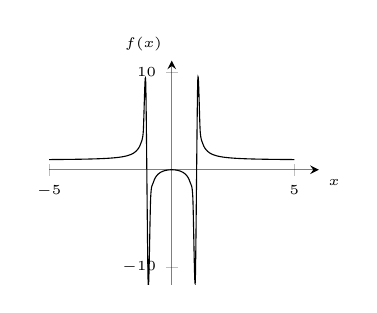
\begin{tikzpicture}
		    \begin{axis}[scale=.5,draw opacity =.5,samples=100,smooth, 
		      axis x line=center, 
		      axis y line=center,
		      ylabel = {$f(x)$},
		      xlabel = {$x$},
		      xlabel style={below right},
		      ylabel style={above left},
		      label style={font=\tiny},
		      tick label style={font=\tiny},
		      enlargelimits=upper] 
		      \addplot[black,opacity=1]{x^2/(x^2-1)};
		    \end{axis}
		\end{tikzpicture}
		\end{center}
		\vspace{.5cm}

	    %---------- (iv)
	    \item $f(x)=\dfrac{1}{1+x^2}$.\\\\
		Respuesta.-\;
		\begin{center}
		    \begin{tikzpicture}
		    \begin{axis}[scale=.5,draw opacity =.5,samples=100,smooth, 
		      axis x line=center, 
		      axis y line=center,
		      ylabel = {$f(x)$},
		      xlabel = {$x$},
		      xlabel style={below right},
		      ylabel style={above left},
		      label style={font=\tiny},
		      tick label style={font=\tiny},
		      enlargelimits=upper] 
		      \addplot[black,opacity=1]{1/(1+x^2)};
		    \end{axis}
		\end{tikzpicture}
		\end{center}
		\vspace{.5cm}
	\end{enumerate}

    %------------------ 4.
    \item 
	\begin{enumerate}[(a)]

	    %---------- (a)
	    \item Si $a_1<\ldots < a_n$ halle el valor mínimo de $f(x)=\sum\limits_{i=1}^n (x-a_i)^2$.\\\\
		Respuesta.-\;

	    %---------- (b)
	    \item 

	\end{enumerate}

\end{enumerate}
